Conside ahora un gas ideal de $2 \mathrm{~N}$ moléculas que se encuentra en un volumen dividido en dos partes iguales: izquierda y derecha, como muestra la figura. Por simplicidad, solo vamos a considerar dos estados de posición: izquierda y derecha. En equilibrio, y en el ensamble microcanónico, cada molécula tiene igual probabilidad de estar a la derecha o a la izquierda. Bajo estas condiciones, ¿cuál es la probabilidad de encontrar $2 \mathrm{~m}$ moléculas más a la izquierda que a la derecha?

Si las moléculas son distinguibles, hay un total de $2^{2 \mathrm{~N}}$ posibles configuraciones del sistema total, cada una con probabilidad $p_i=1 / 2^{2 N}$. De estas, $\left(\begin{array}{c}2 N \\ N+m\end{array}\right)$ configuraciones son compatibles con el estado descrito en la figura. Por lo tanto, la probabilidad de hallar $2 \mathrm{~m}$ moléculas más en la mitad derecha que en la izquierda es
$$
P_m=\frac{1}{2^{2 N}}\left(\begin{array}{c}
2 N \\
N+m
\end{array}\right)
$$
A partir de este resultado,
\begin{figure}
    \centering
    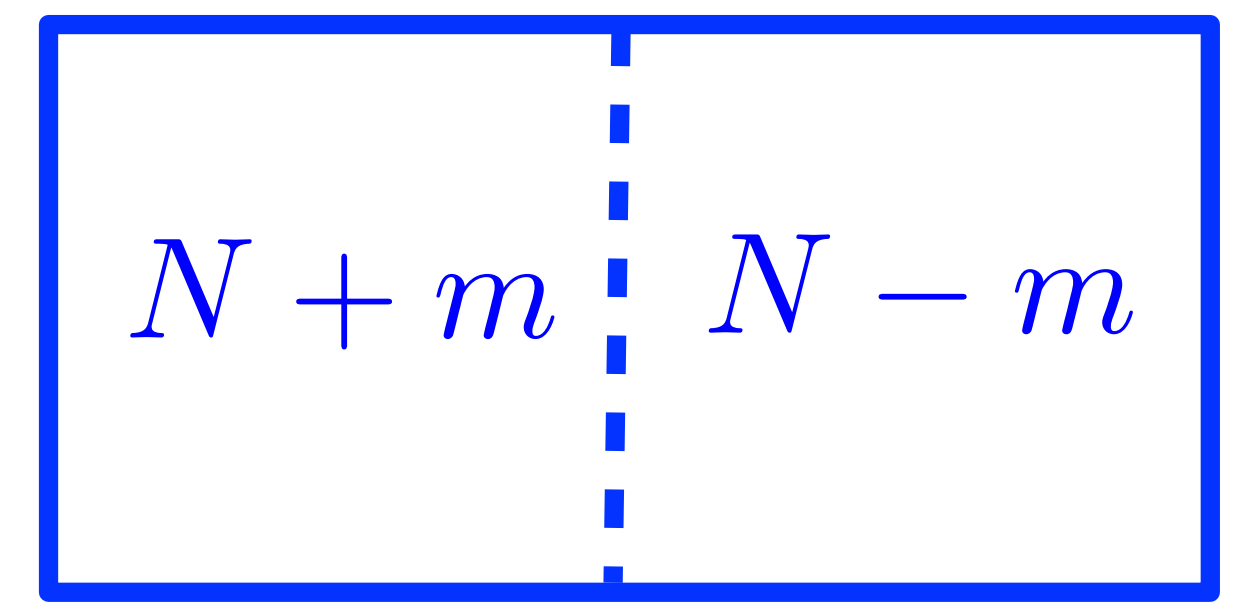
\includegraphics[width=0.5\textwidth]{punto2/cajadividaen2.png}
    \caption{Sistema de $2N$ moleculas dividido en dos partes iguales.}
    \label{fig:my_label}
\end{figure}